\setcounter{topnumber}{5}
\setcounter{bottomnumber}{5}
\setcounter{totalnumber}{5}

\chapter{Problemas propostos}

\section{Problema 1.1.24}
Suponha que um buraco tenha sido feito através do centro da Terra, atravessando-a de ponta a ponta, e uma bola de boliche com massa $m$ seja jogada no buraco, conforme mostra a figura abaixo. Construa um modelo matemático que descreve o movimento da bola. Em um dado instante $t$, seja $r$ a distância do centro da Terra até a massa $m$, $M$ a massa da Terra, $M_{r}$ a massa da parte da Terra dentro de uma esfera de raio $r$ e $\delta$, a densidade constante da Terra. \\

\centerline{\begin{minipage}[c]{\textwidth}
		\centering
		\noindent
		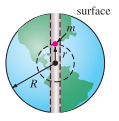
\includegraphics[width=0.3\textwidth]{imagem.png}
		\label{}
\end{minipage}}
\subsection{Problematização}
Devemos construir um modelo matemático que relacione o movimento que a bola de boliche, em queda, em um instante t á uma distância r do centro da terra.

\subsection{Dados}
\begin{center}
	\noindent $m= $\textit{ massa da bola de boliche\\}
	\noindent $M=$\textit{ massa da Terra\\}
	\noindent $r=$\textit{ distância entre a bola e o centro da Terra\\}
	\noindent $M_{r}=$\textit{ massa dentro do raio\\}
	\noindent $R=$\textit{ raio da Terra\\}
	\noindent $\delta = $\textit{ densidade constante da Terra\\}
\end{center}


\subsection{Construção do modelo}
Partindo da segunda lei de Newton, a qual afirma que a força resultante que atua sobre um corpo é proporcional ao produto da massa pela aceleração por ele adquirida. Logo:
\begin{equation}\label{eq1}
F_{r} = m \cdot a
\end{equation}
É conhecido também, que a aceleração pode ser obtida a partir da derivada da velocidade em relação a um instante t, que por sua vez é a derivada de um espaço r em relação a um instante t. Assim, podemos definir a aceleração de um corpo, como a derivada de segunda ordem de r em relação a t:\\

\begin{equation}\label{eq2}
a = \frac{d^{2}r}{dt^{2}}
\end{equation}

\noindent Aplicando (\ref{eq2}) em (\ref{eq1}), obtém-se:
\begin{equation}\label{eqf}
F_{R} = m \cdot \frac{d^{2}r}{dt^{2}}
\end{equation}

\noindent Para obtermos as respectivas massas, podemos valer-nos da seguinte característica intrínseca dos sólidos:
\begin{equation*}
d= \frac{M}{V}
\end{equation*}

\noindent Onde $d$ é a densidade do sólido, $M$ a massa e $V$ o volume do mesmo.
Logo:
\begin{equation*}
M = d \cdot V
\end{equation*}
\noindent Como os objetos em questão possuem formato esférico, teremos:
\begin{equation*}
V = \frac{4\pi R^{3}}{3}
\end{equation*}

\noindent Assim:
\begin{equation}\label{eq3}
M = \frac{4\pi R^{3}}{3} \cdot \delta \rightarrow M_{r} = \frac{4\pi R^{3}}{3} \cdot \delta
\end{equation}

\noindent Para fins de simplificação, podemos fazer o seguinte:
\begin{equation}\label{eq4}
M = \frac{4\pi R^{3}}{3} \cdot \delta \rightarrow 4\pi \delta = \frac{3M}{R^{3}}
\end{equation}

\noindent Aplicando \eqref{eq4} em \eqref{eq3}, obteremos:
\begin{equation*}
M_{r}= \frac{M \cdot r^{3}}{R^{3}}
\end{equation*}

Baseado na lei de gravitação universal, formulada por Isaac Newton, podemos afirmar que força de atração gravitacional entre dois corpos é diretamente proporcional a massa dos corpos em questão e inversamente proporcional ao quadrado da distância entre os dois corpos.
\begin{equation*}
F_{G} = G \cdot \frac{m_{1} \cdot m_{2}}{r^{2}}
\end{equation*}

\noindent A força gravitacional entre $m$ e $M_{r}$, é dada então por:
\begin{equation*}
F_{G} = G \cdot \frac{m \cdot \frac{M \cdot r^{3}}{R^{3}}}{r^{2}} \rightarrow F_{G} = G \cdot \frac{m \cdot M \cdot r^{3}}{R^{3} \cdot r^{2}}
\end{equation*}

\begin{equation}\label{eq5}
F_{G} = G \cdot \frac{m \cdot M \cdot r}{R^{3}}
\end{equation}

\noindent Agora, pode-se fazer uma relação de igualdade entre as forças \eqref{eqf} e \eqref{eq5}:
\begin{equation*}
F_{R} = F_{G}
\end{equation*}
\begin{equation*}
m \cdot \frac{d^{2}r}{dt^{2}} = G \cdot \frac{m \cdot M \cdot r}{R^{3}}
\end{equation*}
\begin{equation}\label{eq6}
\boldmath
\frac{d^{2}r}{dt^{2}} = G \cdot \frac{M \cdot r}{R^{3}}
\end{equation}

\textbf{A \autoref{eq6} é o modelo matemático que relaciona as grandezas necessárias, a uma distância $r$ e um instante $t$.}

\section{Problema 1.3.23}
Na teoria de aprendizagem, supõe-se que a taxa segundo a qual um assunto é memorizado é proporcional à quantidade a ser memorizada. Suponha que M denote a quantidade total de assunto a ser memorizado e $A(t)$ a quantidade memorizada no instante $t$ > 0. Determine uma equação diferencial para a quantidade $A(t)$.

\subsection{Dados}
\begin{center}
	\noindent $M= $\textit{ assunto total a ser memorizado\\}
	\noindent $A(t)=$\textit{ quantidade memorizada, num instante $t > 0$\\}
\end{center}
\subsection{Lógica e modelagem}
O primeiro passo é estipular uma constante de aprendizagem, tendo em vista que existem diferentes formas e níveis de aprendizagem. Essa constante é uma constante usual que torna o valor da E.D.O o mais próximo do real quanto seja possível.
\begin{center}
	\noindent $k= $\textit{ constante proporcional de aprendizagem\\}
\end{center}

Pensa-se agora nas relações e correlações entre os dados acima citados e, ainda, na utilidade dessas relações para a modelagem matemática deste problema.

\textit{“A taxa segundo a qual um assunto é memorizado é proporcional à quantidade a ser memorizada. ”}
Logo:
\begin{equation*}
\frac{dA}{dt} \propto M
\end{equation*}

Porém, deve se notar que $A(t)$ denota quantidade já memorizada – num instante $t$; assim, a medida que $A(t)$ cresce (quando $t>0$) o total de assunto a ser memorizado decresce. Decrescendo junto, assim, a taxa de memorização.
Para fins de entendimento, podemos fazer a seguinte projeção:
\[ \lim_{t \to t_{0}} A(t) = M \]
Onde $t_{0}$ é o instante em que todo o assunto já foi memorizado.
Tomando todas essas hipóteses, é fácil montar uma relação; a quantidade memorizada será proporcional a diferença entre o total que deve ser memorizado e a quantidade já memorizada, adicionando uma constante de proporcionalidade.
\begin{equation}\label{eqmemo}
\boldmath
	\frac{dA}{dt} = k(M-A(t))
\end{equation}

\section{Problema 1.3.23}
\subsection{Lógica e modelagem}
Assim como o problema anterior, devemos estipular uma constante de proporcionalidade, afim de obter resultados próximos a realidade:
\begin{center}
	\noindent $c= $\textit{ constante proporcional de esquecimento\\}
\end{center}
Percebendo que \textit{“a taxa segundo a qual o assunto é esquecido seja proporcional à quantidade memorizada no instante $t > 0$”}, podemos afirmar que a taxa de esquecimento cresce juntamente a quantidade já memorizada ($A(t)$) e é uma grandeza que se opõe ao total de assunto a ser memorizado ($M$).
Tomando a modelagem anterior como uma verdade podemos apenas acrescentar a taxa de esquecimento na modelagem da problematização anterior:
\begin{equation}
\boldmath
\frac{dA}{dt} = k(M- A(t)) - c(A(t))
\end{equation}